\chapter{Ad-hoc Information Retrieval}
\label{ch:ir}

Topic models explore and summarize document collections outside the context of any specific information need, when we do not necessarily know what we are looking for.
This approach to information retrieval stands in contrast to traditional IR systems, which retrieve relevant documents given users' explicit information needs.
Where IR systems might look for the ``needle in the haystack'', topic models will tell you about the overall proportion of hay and needles, and perhaps inform you about the mice that you did not know were there.
But topic models can also be useful in situations when we do have a specific information need, but we do not quite know how to search for it.
Despite their differences in purpose, there are strong mathematical and conceptual connections between these two approaches.
In this chapter we consider the use of topic modeling in IR to balance specific user queries with more open-ended discovery.

In the most direct sense, topic models can be used as a simple indexing method.
Users can find topics that assign high probability to a particular query term, and then find documents that exhibit a high probability of these topics.
Such topic-based search may additionally provide some level of query disambiguation, since it may be clear from topic-word distributions that one or another topic is more relevant to the user's information need.
More sophisticated approaches blur the boundary between query-driven retrieval and unsupervised topic modeling.
\citet{erlin2017topic} search for passages related to epistemology in English and German books by ``seeding'' topic models with words thought to be relevant to that subject.
This approach can be successful, but does not guarantee that relevant topics will be found, or that topics will really match the intended subject.

In the more formal ad hoc retrieval setting, users start with an information need expressed in the form of one or more queries. Many IR systems treat both the queries and documents as ``bags of words'', and retrieve and rank the documents by measuring the word overlap between queries and documents.
However, the ability of this direct and simple matching is always
limited. Words with similar meaning or in different forms should also
be considered as matched instead of being ignored. \textbf{Language
  modeling} has been one of the most popular frameworks to capture
such semantic relationships. But humans would also like to use background
knowledge to interpret and understand the queries and ``add'' missing
words~\citep{wei-07}, which provides another approach often referred to as
\textbf{query expansion} to improve retrieval and ranking results.

Both directions can be pursued by learning and discovering the
semantic relations between words and, further, the semantic relations
between queries and documents. Topic models provide semantic relations between query words and
documents~\citep{deerwester-90,hofmann-99a} by describing each topic
using probabilistically-weighted words and modeling each document as a distribution over
all topics.
In this way they add a layer of abstraction between a document and the exact words present in that document.
Appealing to the generative ``story'' of a model, we want to recover the words that {\em could} have been available to an author based on the words that were actually chosen.
Such semantic relations
can be applied to smoothing the language models, or introducing
related words in query expansion. This chapter focuses on how to apply
topic models in document language modeling \citep{Lu-2011,wei-06} and
query expansion~\citep{Park-2009,Andrzejewski-2011} to further improve
 ranking results of information retrieval.

\section{Document Language Modeling in IR}
\label{sec:ir-lm}

The language modeling approach~\citep{croft-03,PonteCroft,song-99} is
one of the main frameworks for using topic models in IR systems, since
it has been shown to be an effective probabilistic framework for studying
information retrieval problems~\citep{PonteCroft,berger-99}.
A statistical language model estimates the probability of word
sequences, denoted as $p(w_1,w_2,\cdots,w_n)$. In practice, the
statistical language model is often approximated by N-gram models. A
unigram model assumes each word in the sequence is independent, and is
denoted as,
\begin{align}
p(w_1,w_2,\cdots,w_n) = p(w_1)p(w_2) \cdots p(w_n)
\end{align}
A trigram model assumes the probability of the current word only
depends on the previous two words, and it is represented as
\begin{align}
p(w_1,\cdots,w_n)=p(w_1)p(w_2|w_1)p(w_3|w_1,w_2)\cdots p(w_n|w_{n-2},w_{n-1})
\end{align}

In the application of information retrieval, the queries are generated
by a probabilistic language model based on a
document~\citep{zhai-01}. More specifically, each document is viewed
as a language sample, and a language model for each document is
estimated based on document terms. Then the
probability of generating a query is estimated by multiplying the probabilities of
generating each query term using a document language model,
and the documents are ranked based on the probability.

Given a document sample $d$, a straightforward way to estimate the
probability of generating a word $w$ is to use maximum likelihood
estimation
\begin{align}
p_{\texttt{ml}}(w \g d) = \frac{n_{d,w}}{n_{d,\cdot}}
\label{eq:ir_mse}
\end{align}
where $n_{d,w}$ is the term frequency of word $w$ in document $d$, and
$n_{d,\cdot}$ is the total number of tokens in document $d$. Then the
probability of generating the given query $q$ is
\begin{align}
p(q \g d) = \prod_{w \in q} p(w \g d) = \prod_{w \in q} \frac{n_{d,w}}{n_{d,\cdot}}
\end{align}

Then the documents are ranked based on this probability $p(q \g d)$. Higher
probability implies the corresponding document is more relevant to the
given query~\citep{song-99}. However, a document often contains limited number of words and
maximum likelihood estimation gives zero probability to those unseen words.
If a query contains any word that is not included in the document, the probability
of generating the whole query given this document is zero, which may throw out perfectly good documents.

This data sparsity problem can be fixed by smoothing, which allocates
some non-zero probability to the missing terms. In fact, topic models
provide a unique way to extract the word probabilities given the
corpus, which can be used to smooth document language models.  In
this section, we summarize two simple smoothing methods, and then
show how topic models fit into this smoothing framework.

%\subsection{Smoothing Document Language Models}

\jbgcomment{Is this important to talk about here?  I worry that it
  might be a distraction.  will this connect directly to topic models?
  \yhcomment{Yes, it is important. Topic models are applied to
    document LM in forms of smoothing. Simplified and added more
    connections. }}

There are two major directions for smoothing:
\textbf{interpolation}~\citep{Jelinek-1980,mackay95dirichlet,Ney-1994,PonteCroft,zhai-01}
and \textbf{backoff}~\citep{katz-87,song-99}. The interpolation-based
method discounts the counts of the seen words and distribute the extra
counts to both seen words and unseen words. An alternative backoff
smoothing strategy trusts the maximum likelihood estimation for high
count words, discounts and redistributes mass only for the less common
words~\citep{zhai-01}.

Here we introduce two popular and simple interpolation smoothing
methods, which are further used by topic models to smooth document
language models.

\paragraph{Jelinek-Mercer method}

The Jelinek-Mercer method~\citep{Jelinek-1980} is a linear
interpolation of the maximum likelihood model in a document with the
model based on the whole corpus, and a coefficient $\lambda$ is used
to combine the two parts.
\begin{align}
p(w|d) = (1 - \lambda) p_{\texttt{ml}}(w|d) + \lambda p(w|\mathcal{C})
\label{eq:lm-jr}
\end{align}
where $\mathcal{C}$ denotes the whole corpus. This simple mixture
solves the data sparsity problem. For terms that occur in the document
$d$, the maximum likelihood estimator (Equation~\ref{eq:ir_mse}) is
not accurate given the limited size of a document, thus it is smoothed
with the more reliable corpus level probability. For a missing term $w$
in the document $d$, the probability of generating word $w$ is not zero any more, but falls
back to the corpus level probability $p(w|\mathcal{C})$.
This smoothing method has been explored and successfully applied in information retrieval tasks~\citep{PonteCroft,song-99}.

%This smoothing method has been explored by \cite{PonteCroft} and \cite{song-99} in information retrieval task, except \cite{PonteCroft} explored a weighted product version instead of a linear interpolation.
%\begin{align}
%p(w|d) = p_{\texttt{ml}}(w|d)^{(1 - \lambda) } \times p(w|\mathcal{C})^{\lambda}
%\label{eq:lm-jr}
%\end{align}
%But in general, the linear interpolation is more popular since the resulting probability is still normalized~\citep{song-99}.

\paragraph{Bayesian Smoothing using Dirichlet Priors}

A language model can be viewed as a multinomial distribution, thus it
can be smoothed by applying the Dirichlet distribution as the
conjugate prior~\citep{mackay95dirichlet}. This smoothing model is
adding an extra prior count for each word to smooth the probability of
unseen words,
\begin{align}
p(w \g d) = \frac{n_{d,w} + \beta p(w|\mathcal{C})}{\sum_{v \in V} n_{d,v} + \beta}
\end{align}
where the Dirichlet prior is decided by concentration parameter $\beta$ and the
corpus-level probabilities $p(v|\mathcal{C})$
\begin{align}
(\beta p(v_1 \g \mathcal{C}), \beta p(v_2 \g \mathcal{C}), \cdots, \beta p(v_n \g \mathcal{C}))
\label{eq:lm-bs}
\end{align}

%\paragraph{Absolute Discounting}

%Absolute discounting is to allocate some probability mass from the
%seen words to the unseen words~\cite{Ney-1994}. Normally, a constant
%is subtracted from their actual counts for the seen words. This model
%is given by, \begin{align} p(w|d) = \frac{\max(n_{d,w} - \delta,
%0)}{\sum_{v \in V} n_{d,v}} + \sigma p(w|\mathcal{C}) \end{align}
%where $\delta \in [0,1]$ is the discount constant and $\sigma =
%\delta n'_{d,\cdot} / n_{d, \cdot}$, $n_{d, \cdot}$ is the total
%number of tokens in document $d$, and $n'_{d,\cdot}$ is the number of
%unique terms in document $d$.

\section{Applying Topic Models to Document Language Models}

Topic models, which model each document as a mixture of topics and
each topic as a mixture of words, offer an interesting framework to
model documents in information retrieval. Popular topic models such as
probabilistic Latent Semantic Analysis~(\abr{plsa}) and Latent Dirichlet Allocation (\abr{lda})
have been both explored to improve document language models.

\cite{hofmann-99a} first introduces \abr{plsa} to
to learn the relationship between query words and documents,
and the conditional probability of a query word $w$ given a document $d$ is
computed as marginalizing all topics $k$,
\begin{align}
p_{\texttt{TM}}(w|d) = \sum_{k} p(w \g k) p(k \g d)
\end{align}

Later, \cite{wei-06} apply the same idea to learn the topic-smoothed document-word
distribution, using \abr{lda} instead of \abr{plsa}.
Because topic models learn the semantic relationships between words
and documents through learning the hidden topics and their posterior
estimates of document-topic distribution and topic-word distribution
are smoothed by the Dirichlet priors, topic models learn a better and
smoothed semantic relationship between document words and documents. However,
while the original document language model directly models the relationship
between query words and documents, the topic models based on documents only 
lose the relationship between query words and documents,
but it is a good approach to complement the original document
language models. Thus \cite{wei-06} further propose to combine the
\abr{lda}-based document model with the original smoothed document
model~(Equation~\ref{eq:lm-jr}) through a linear interpolation,
\begin{align}
p(w \g d) = \lambda' \Big( (1 - \lambda) p_{\texttt{ml}}(w|d) + \lambda
p(w \g \mathcal{C}) \Big) + (1 - \lambda') p_{\texttt{TM}}(w|d)
\end{align}
where $\lambda'$ is the coefficient which combines the LDA-based
document model with the general smoothed language model.

Following \cite{wei-06}, \cite{Lu-2011} further evaluate the
performance of applying topic models into the document language model
framework. Instead of combining with the language model with
Jelinek-Mercer smoothing~(Equation~\ref{eq:lm-jr}), \cite{Lu-2011}
smooth the document language model with Bayesian
smoothing~(Equation~\ref{eq:lm-bs}), and the final linear combination
with topic models
\begin{align}
p(w \g d) = \lambda \frac{n_{d,w} + \beta p(w \g \mathcal{C})}{\sum_{v
  \in V} n_{d,v} + \beta}  + (1 - \lambda) p_{\texttt{TM}}(w \g d)
\end{align}

While using different smoothing strategies, both
approaches~(\citep{wei-06} and \citep{Lu-2011}) apply topic models to
connect the query words with documents through hidden topics. As a
result, better semantic relationships between query words and
documents can be learned to complement the document language models.

\jbgcomment{Would be good to have an example of how this works.}

\section{Query Expansion in IR}

The document language models in information
retrieval~\citep{PonteCroft} have been attempting to model the query
generation process based on the document models. However, a big
problem is that these models abandon modeling the query-document
relevance explicitly~\citep{Lavrenko-2001}, which is very important in
traditional information retrieval task.

In fact, queries, which are normally brief and using informal
languages from users, diverge significantly from the language in
documents~\citep{Muller-2009}. This semantic gap or lexical gap can
result in poor query-document relevance, even though the document is
quite relevant from the users' view point. This is due to users, who
add ``missing'' or potentially related words implicitly in their minds
and then consider the query-document relevance.

Query expansion simulates a similar process. Query expansion
normally analyzes the relationships between the query words and other
words, and tries to find potential related words so that the original
query is better represented and better query-document relevance can be
obtained. For example, without much context, it would be really hard 
to understand what a query ``dtd amc'' means~\citep{Jiang-2016}. Through
query expansion, it is possible to build up the relationship between ``dtd''
and ``disneyland downtown'', which is more helpful in document retrieval. 
Next, this section reviews the classic query expansion frameworks
in information retrieval, and the related works about using topic models
for query exapansion are introduced in the next section.

\subsection{Learning Query-Word Relationships for Query Expansion}

There are two main steps for query expansion. The first step is to
find the relationships between queries and words and select the top
related words to expand the query. The second step is to apply the
expanded queries for ranking and compute the final ranking relevance
scores. We start with the first step. Two major directions have been
explored: query language model~\citep{zhai-01b} and relevance
model~\citep{Lavrenko-2001}.

\paragraph{Query Language Model}

To learn the query-word relationship, \cite{zhai-01b} build up a query
language model to estimate the probability $p(w \g q)$ of a word $w$
given a query $q$. However, it is not easy to learn a good query
language model since the query content is too limited.

\cite{zhai-01b} propose to use both the query content and the relevant
documents $\mathcal{F}$ (sometimes referred as feedback documents or clicked
documents) to estimate the query language model. Let
$\hat{\theta}_{\mathcal{F}}$ be the estimated query language model
based on the relevant documents and $\hat{\theta}_{Q}$ is the original query language model estimated purely based on queries,
the combined query model $\hat{\theta}_{Q'}$ is
\begin{align}
\label{eq:qlm-comb}
\hat{\theta}_{Q'} = (1 - \lambda)\hat{\theta}_{Q} + \lambda \hat{\theta}_{\mathcal{F}}
\end{align}

Estimating $\hat{\theta}_{Q}$ is obvious based on query words, and $\hat{\theta}_{\mathcal{F}}$ can
also be simply estimated by a unigram language model $\theta$
which generates each word in $\mathcal{F}$ independently. However,
most documents contain not only the query relevant information, but
also the background information. As a result, \cite{zhai-01b} propose
to generate a relevant document by a mixture model, which combines a
language model $p(w|\theta)$ with a collection language model
$p(w|\mathcal{C})$, and the log-likelihood of the relevant document
is,
\begin{align}
\log p(\mathcal{F}|\theta) = \sum_i \sum_w n_{d_i, w} \log((1-\lambda')p(w|\theta) + \lambda' p(w|\mathcal{C}))
\end{align}
where $n_{d_i, w}$ is count of word $w$ in document $d_i$. The related parameters $\theta$ are estimated by the EM algorithm (more details can be found in \cite{zhai-01b}). By combing with the information from the relevant documents, the query language model is more robust, thus query-word relationships are better represented.

\paragraph{Relevance Model}

Unlike the query language model approach~\citep{zhai-01b},
\cite{Lavrenko-2001} assume both the query and the relevant documents
are random samples from an unknown relevance model $R$. Given the
query $q$, they approximate the probability $p(w|R)$ based on the
observed query $q$ as the following,
\begin{align}
p(w|R) \approx p(w|q) = \frac{p(w,q)}{p(q)}
\end{align}

To estimate the joint probability $p(w,q)$, \cite{Lavrenko-2001}
assumes the word $w$ and the query $q$ are sampled independently from
the same distribution, e.g., from a unigram distribution, then the
joint probability can be computed as,
\begin{align}
p(w, q) = \sum_{d \in \mathcal{C}} p(d) p(w,q |d) = \sum_{d \in \mathcal{C}} p(d) p(w|d) p(q | d)
\end{align}

Then the multinomial distribution $p(w|q)$ for a given query $q$ can
be computed as follows,
\begin{align}
\label{eq:rm_qe}
p(w|q) = \frac{p(w, q)}{p(q)} = \sum_{d \in \mathcal{C}} p(w|d) p(d|q)
\end{align}

Both the query language model and the relevance model capture the
relationship between the query and other words, based on which the top
related words can be selected for query expansion.

\subsection{Ranking Relevance with Query Expansion}

Given the related words for query expansion, the next question is how
to apply the expanded queries for computing the final ranking
relevance score. The combination can happen either before or after the
relevance score is computed.

\cite{zhai-01b} combine the expanded query language model
$\hat{\theta}_{\mathcal{F}}$ with the original query language model
$\hat{\theta}_{Q}$ as one query language model $\hat{\theta}_{Q'}
$~(Equation~\ref{eq:qlm-comb}). Given a query $q$ generated from the
expanded query model $p(q|\hat{\theta}_{Q'})$, and a document $d$
generated from a document model $p(d|\hat{\theta}_D)$, they compute
the KL-divergence of document $d$ with respect to query $q$ as the
final relevance score:
\begin{align}
\label{eq:KL}
D(\hat{\theta}_{Q'} || \hat{\theta}_D) = -\sum_w p(w|\hat{\theta}_{Q'}) \log p(w | \hat{\theta}_D) + \texttt{cons}(q)
\end{align}

In contrast to \cite{zhai-01b}, \cite{Lavrenko-2001} compute
the relevance score using the original query and the expanded query
respectively, and then linearly combine the two scores. Thus the final
query-document relevance $\hat{s}_d(q)$ is computed as,
\begin{align}
\label{eq:rm_qe_comb}
\hat{s}_d(q) = \lambda s_d(e) + (1-\lambda)s_d(q)
\end{align}
where $s_d(q)$ is the relevance between the original query $q$ and
documents $d$, and $s_d(e)$ is relevance between the expanded query
terms $e$ and document $d$.

\section{Applying Topic Models For Query Expansion}

Topic models capture the semantic relationships of words through
learning the latent topics, which are presented as distributions over
different words. Such semantic relationships among words provide a
unique way to match or expand words at the semantic level rather than
by a direct spelling matching. For example, given a short query ``diabetes'',
topic models can easily find the related words such as
``insulin'', ``glucose'', ``coronary'' and ``metformin'' etc., 
as they often occur in the same context~\citep{Zeng-2012}. 
As a result, topic models have been
successfully applied into query expansion~\citep{Yi-2009,Park-2009,Zeng-2012}.

\paragraph{Smoothing Query Language Model}

The most intuitive way to apply topic models for query expansion is to
extract the words' relevance from topics directly as
\cite{Yi-2009}. They train a topic model, from which the probability
$p_{\texttt{TM}}(k|q)$ of a topic $k$ in a query $q$ is learned. Then
the query-word relevance $p(w|q)$ is computed based on topics as
follows,
\begin{align}
\label{eq:query_word_prob}
p(w|q) = \sum_k p_{\texttt{TM}}(w|k) p_{\texttt{TM}}(k|q)
\end{align}

This query-word relevance $p(w|q)$ from topic models can be used to
smooth the original query language model through linear
interpolation. However, queries are normally too short to learn
meaningful topics, thus the quality of query-word relevance is
relatively limited. To improve the quality of extracted topics,
\cite{Yi-2009} also train topic models from the relevant documents
(e.g., top documents retrieved by a query), and extract the query-word
relationships based on the Equation~\ref{eq:query_word_prob} for query
expansion.

\paragraph{Improving Relevance Model}

In addition to this direct approach, \cite{Yi-2009} also apply topic
models to improve the relevance model in Equation~\ref{eq:rm_qe} for
query expansion. In this approach, topic models are applied to capture
the document-word relationship $p(w|d)$ given the query $q$ as
follows,
\begin{align}
p_{\texttt{TM}}(w|d,q) = \sum_k p(w|k) p(k|d,q)
\end{align}
where,
\begin{align}
%p(k|d,q) &= \frac{p(k,d,q)}{p(d,q)}  = \frac{p(k)p(d|k)p(q|k)}{p(d,q)} \\
%&= \frac{p(k|d)p(q|k)}{p(q|d)} \approx p(k|d)p(q|k) \notag
p(k|d,q) = \frac{p(k|d)p(q|k)}{p(q|d)} \approx p(k|d)p(q|k)
\end{align}
where $p(k|d)$ is the topic probability in document $d$, and $p(q|k)$
is the probability of generating a query $q$ given the topic $k$. Then
the topic-based document-word relationship $p_{\texttt{TM}}(w|d,q)$ is
applied to smooth the document-word relationship $p(w|d)$ in the
relevance model~(Equation~\ref{eq:rm_qe}) through a linear
interpolation,
\begin{align}
p(w|q) = \sum_{d \in \mathcal{C}} (\lambda p(w|d) + (1 - \lambda)p_{\texttt{TM}}(w|d,q))p(d|q)
\end{align}
where $\lambda$ is a constant weight to combine the original relevance
model and the topic-based relevance model. Because the topic models
capture the word relationships on a semantic level, this improved
relevance model better captures the query-word relationships and
improve query expansion.

\paragraph{Learning Pair-wise Word Relationships}

\cite{Park-2009} also apply topic models for query expansion but in a
different way. They model the pair-wise relationships between words
through topic models and then apply it for query expansion. More
specifically, based on the topics extracted from topic models, they
compute the probabilistic relationships of each word pair $(w_x,
w_y)$,
%\begin{align}
%p(w_x|w_y, \alpha) &= \sum_i p(w_x, z_i | w_y, \alpha) \\
%&= \sum_i p(w_x | z_i, w_y, \alpha) p(z_i | w_y, \alpha) \notag\\
%&= \sum_i p(w_x|z_i, \alpha) p(z_i|w_y, \alpha) \notag
%\end{align}
\begin{align}
p(w_x \g w_y, \alpha) &= \sum_k p(w_x, k  \g  w_y, \alpha) \\
%&= \sum_k p(w_x  \g  k, w_y, \alpha) p(k  \g  w_y, \alpha) \notag\\
&= \sum_k p(w_x  \g  k, \alpha) p(k  \g  w_y, \alpha) \notag
\end{align}
where $\alpha$ is the concentration parameter of the Dirichlet prior
for document-topic distributions and $p(w_x  \g  k, \alpha)$ is the
topic-word distribution which can be learned from topic models, and
$p(k  \g  w_y, \alpha)$ is
%\begin{align}
%p(z_i|w_y, \alpha) &= \frac{p(w_y|z_i,\alpha)p(z_i|\alpha)}{p(w_y|\alpha)} \\
%&= \frac{p(w_y|z_i,\alpha)p(z_i|\alpha)}{\sum_j p(w_y, z_j|\alpha)} \notag\\
%&= \frac{p(w_y|z_i,\alpha)p(z_i|\alpha)}{\sum_j p(w_y|z_i,\alpha)p(z_i|\alpha)} \notag
%\end{align}
\begin{align}
p(k  \g w_y, \alpha) 
%&= \frac{p(w_y  \g  k,\alpha)p(k \g \alpha)}{p(w_y \g \alpha)} \\
%&= \frac{p(w_y|k,\alpha)p(k|\alpha)}{\sum_{k'} p(w_y, k'|\alpha)} \notag\\
&= \frac{p(w_y|k,\alpha)p(k|\alpha)}{\sum_{k'} p(w_y|k',\alpha)p(k' \g \alpha)} \notag
\end{align}
where $p(w_y \g k,\alpha)$ is the topic-word distributions. \cite{Park-2009} also show that $p(k|\alpha) = \frac{\alpha_k}{\sum_j \alpha_j}$.
%\begin{align}
%p(z_i|\alpha) &= \int p(z_i, \theta | \alpha) d\theta \\
%&= \int p(z_i | \theta, \alpha) p(\theta | \alpha) d\theta \\
%&= \int p(z_i | \theta) p (\theta | \alpha) d\theta \\
%& = \mathcal{E}_{p(\theta | \alpha)} [\theta_i]\\
%&= \frac{\alpha_i}{\sum_k \alpha_k}
%\end{align}
As a result, we have,
%\begin{align}
%p(z_i|w_y, \alpha) &= \frac{p(w_y|z_i,\alpha) \frac{\alpha_i}{\sum_k \alpha_k} }{\sum_j p(w_y|z_i,\alpha) \frac{\alpha_j}{\sum_k \alpha_k}} \\
%&= \frac{p(w_y|z_i,\alpha) \alpha_i}{\sum_j p(w_y|z_i,\alpha) \alpha_j} \notag
%\end{align}
\begin{align}
p(k|w_y, \alpha) %&= \frac{p(w_y \g k,\alpha) \frac{\alpha_k}{\sum_j \alpha_j} }{\sum_{k'} p(w_y|k',\alpha) \frac{\alpha_{k'}}{\sum_j \alpha_j}} \\
&= \frac{p(w_y \g k,\alpha) \alpha_k}{\sum_{k'} p(w_y|k',\alpha) \alpha_{k'}} \notag
\end{align}

The final probabilistic relationships of each term pair  can be represented as
%\begin{align}
%p(w_x|w_y, \alpha) = \frac{\sum_i p(w_x|z_i, \alpha) p(w_y|z_i,\alpha) \alpha_i }{\sum_j p(w_y|z_j,\alpha) \alpha_j}
%\end{align}
\begin{align}
p(w_x|w_y, \alpha) = \frac{\sum_k p(w_x|k, \alpha) p(w_y|k,\alpha) \alpha_k }{\sum_{k'} p(w_y|k',\alpha) \alpha_{k'}}
\end{align}

Once this term relationship is obtained, they choose the top related
terms as the expanded terms $e$ for the given query $q$, and the final
document ranking score is computed as Equation~\ref{eq:rm_qe_comb}.

\paragraph{Getting Interactive Feedback}

Relevance feedback involves the users in the retrieval process to improve 
the ranking result set~\citep{Rocchio-1971}. The basic idea is to ask users 
to give feedback on the relevance of documents in an initial set of retrieval 
results, and users' feedback on relevance is further used to improve the 
ranking results. This process can go through one or more iterations.

\cite{Andrzejewski-2011} present a new framework for obtaining and
exploiting user feedback at the latent topic level. They learn the
latent topics from the whole corpus and construct meaningful topic
representations. At query time, they decide which latent topics are
potentially relevant and present the topic representations along
keyword search results. When a user select a latent topic, the
original query is expanded with the top words in this selected topic,
and the search results are refined. 
Query ``euro opposition'' is used as an example in \cite{Andrzejewski-2011},
and the users want to find documents about opposition to the introduction of
the single European currency. 500 topics are learned using the corpus and relevance
judgements. 7 of the 500 topics are selected to show to users as shown in
Table~\ref{tab:topic-feedback} and the user select the Topic 79 as the user feedback.
Using the top 10 terms in Topic 79 as the expanded query terms, the ranking of
the relevant documents has been significantly improved.

\begin{table}[!tp]
\begin{center}
\footnotesize
\setlength\tabcolsep{3pt}
\begin{tabular}{c  p{9cm} } \hline
Topic & Terms \\ \hline \hline
196 (debate) & Tory Euro sceptics, social chapter, Liberal Democrat, mps, Labour, bill, Commons \\
404 (ratification) & ratification Masstricht treaty, Poul Schluter, Poul Rasmussen, Danish, vote, Denmark, ec \\
\textbf{79 (Emu)} & economic monetary union, Masstricht treaty, member states, European, Europe, Community, Emu \\
377 (George) & President George Bush, White House, Mr Clinton, administration \\
115 (power) & de regulation bill, Sunday trading, Queen Speech, law, legislation, government, act \\
446 (years) & chairman chief executive, managing director, finance director, Sir, board, group, company \\
431 (cabinet) & Mr John Major, prime minister, Mr Major, party, tory, government, Conservative \\
\hline
\end{tabular}
\caption{Given query ``euro opposition'', seven topics are selected and shown to a user. The user selected Topic 79
as the feedback topic (Example from \citet{Andrzejewski-2011}).}
\label{tab:topic-feedback}
\end{center}
\end{table}

This direction is actually more related to topic labeling and iterative visualization f
or topic models, which will be further discussed in Chapter~\ref{ch:viz}.

%In order to construct more meaningful topic representations,
%\cite{Andrzejewski-2011} extract multiple features, such as word
%probability, topic posterior, PMI, etc., and then select a single
%best topic word for each topic as the topic label. They also identify
%the statistical significant bigrams and trigrams to further better
%represent the topics. In addition, they restore the capitalization
%for the n-grams to ease users' interpretation of topics.

%At run time, given a query and its top ranked documents,
%\cite{Andrzejewski-2011} select the top two topics from the each of
%the top two ranked documents as the enriched topic set. They further
%study the topic relations and identify the top two topics with the
%highest covariance with each enriched topics, which is defined as the
%related topics. They also filter out the in-coherent topics by using
%PMI scores. For the remaining coherent topics,
%\cite{Andrzejewski-2011} display their unigram, bigram and trigram
%representations to users along the search results of the original
%query. Once a user select a latent topic, the search results are
%updated by expanding the original query with the top words in this
%select topic.

\section{Beyond Relevance---Search Personalization}

Traditional search systems retrieve documents based on the queries only, regardless of who submitted the queries.
As more Web pages become available, queries are normally too short to express users' needs, and
users may prefer different results even the input queries are the same~\citep{Jansen-2000,Dou-2007}.
As the examples shown in \citet{Dou-2007}, the query ``mouse'' may mean ``rodents'' for biologists, 
while the programmers may use the same query to search for computer peripherals. Even for queries without
ambiguity, for example ``online shopping'', some users may prefer ``\url{www.amazon.com}'' while others may
prefer ``\url{www.ebay.com}''.

In order to meet different users' information needs, it is important to understand the user's preference, context,
etc., and adapt the ranking results accordingly~\citep{Pitkow-2002,Micarelli-2007}.
This is referred as personalized search, or search personalization.

There are multiple ways to do search personalization, and two of major directions are normally referred as contextualization~\citep{Melucci-2012} 
and individualization~\citep{Pitkow-2002}. The former is to consider users' conditions in a search activity, for example, time and location.
The latter focuses more on users' individual characteristics and activities, which is also described as the users' profile.
Topic models have been investigated to model users' preference on the topic space~\citep{Song-2010,Carman-2010}.

\paragraph{Modeling Users' Preference via the Output Topics}

\cite{Song-2010} apply topic models to model users' preference from
users' search history. The idea is very similar to smoothing query
language models $p(w \g q)$ by topic models, as explained in Equation~\ref{eq:query_word_prob}. The estimation of $p(w \g q)$ is split into two parts $p(w \g k)$ and $p(k \g q)$.

For each users' query, they concatenate the clicked documents (or the top $n$ ranked documents if no click happened) as a big preference document. Then the topic model pLSI is applied on the preference collection to extract the latent topics as users' preference ($p(w|k)$ in the Equation~\ref{eq:query_word_prob}). The second part is to estimate the query-topic distribution $p(k|q)$ in Equation~\ref{eq:query_word_prob}. However, the queries are too short to estimate the query topics directly. Instead, they first estimate a language model $\theta_q$ from the big preference document of query $q$ and compare the cosine similarity against each topic to estimate the query-topic distribution $p(k \g q)$,
\begin{align}
p(k \g q) = \frac{p(k, q)}{\sum_k p(k, q)} \approx \frac{\text{sim}(\theta_k, \theta_q)}{\sum_k \text{sim}(\theta_k, \theta_q)}
\end{align}

The query language model $p(w|q)$ is further used in the ranking framework with KL divergence~(Equation~\ref{eq:KL}). In this framework, the topics more relevant to the current query and user contribute more to the query model and further bias the ranking results towards users' personal preference.

\paragraph{Encoding Users into Topic Models}

\cite{Carman-2010} also investigate topic models on large query logs for search personalization and propose a personalization topic model as shown in Figure~\ref{fig:ptm-original}. The idea is given the topic distribution of the document, there will be a number of words chosen at random to generate the query and a number of users who chose to click that document.

\begin{figure}
  \begin{center}
  \begin{subfigure}{.5\textwidth}
  \centering
  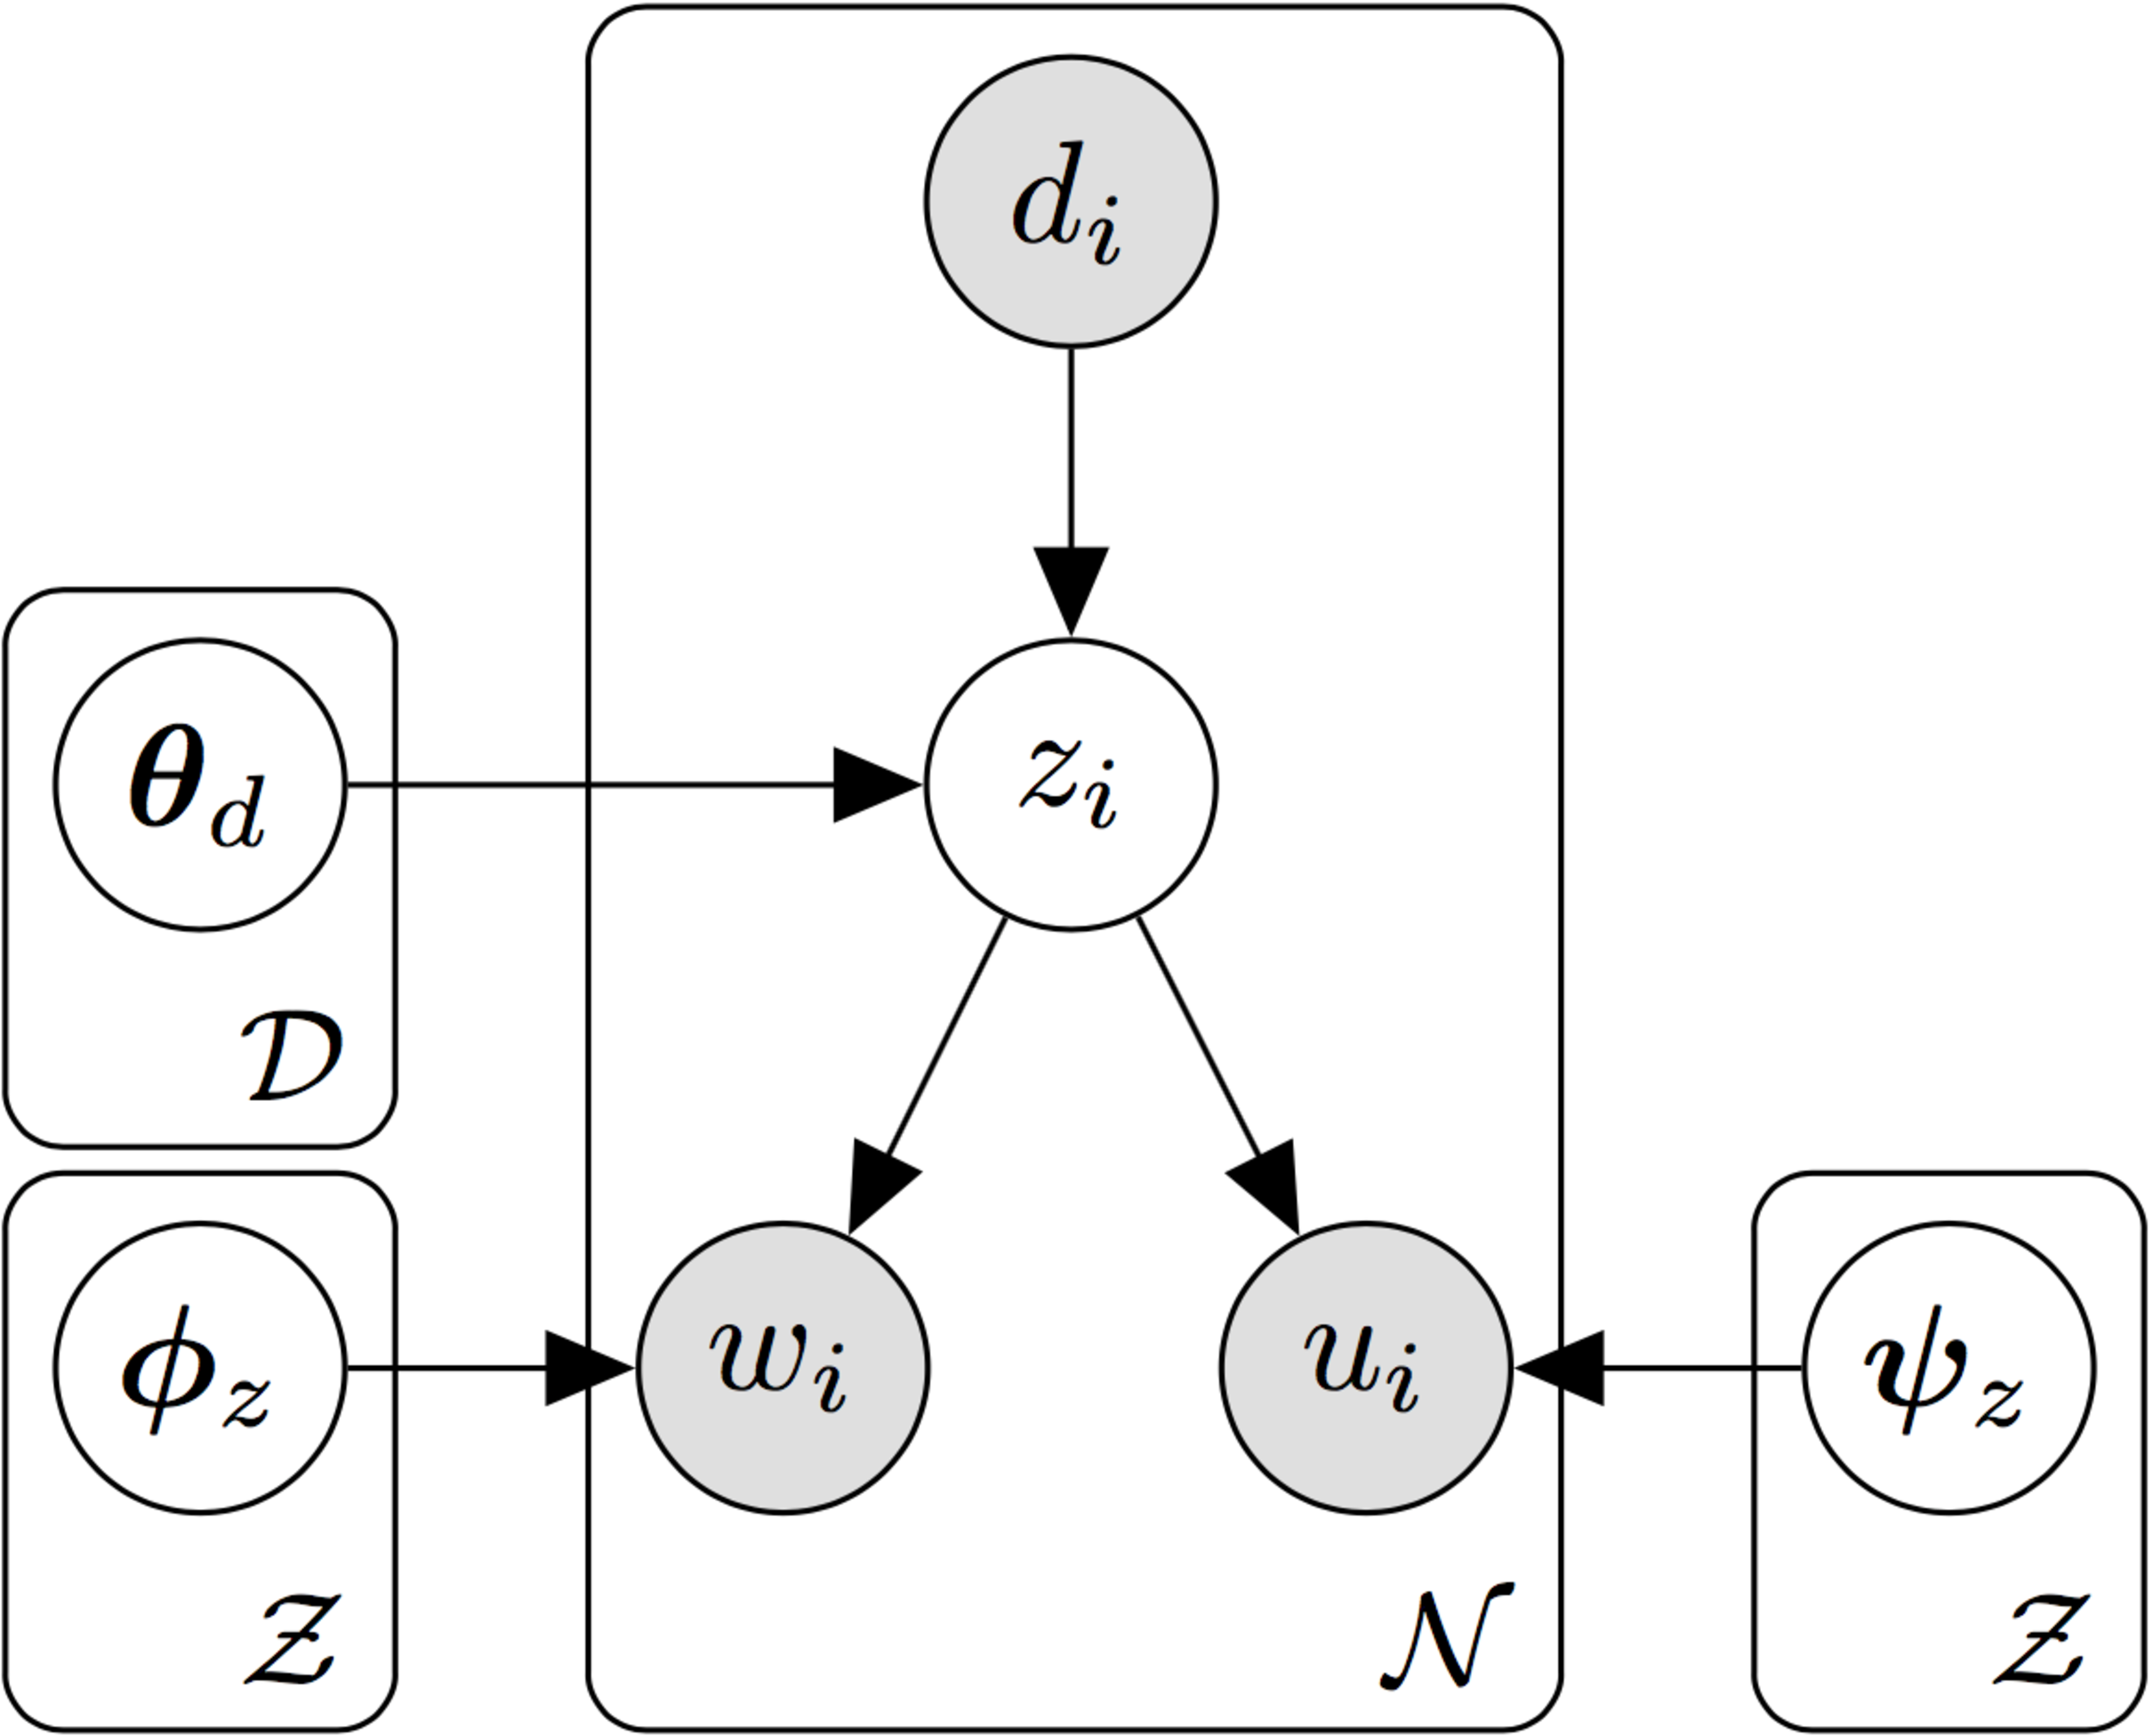
\includegraphics[width=0.8\linewidth]{figures/ptm}
  \caption{}
  \label{fig:ptm-original}
  \end{subfigure}%
  \begin{subfigure}{.5\textwidth}
  \centering
  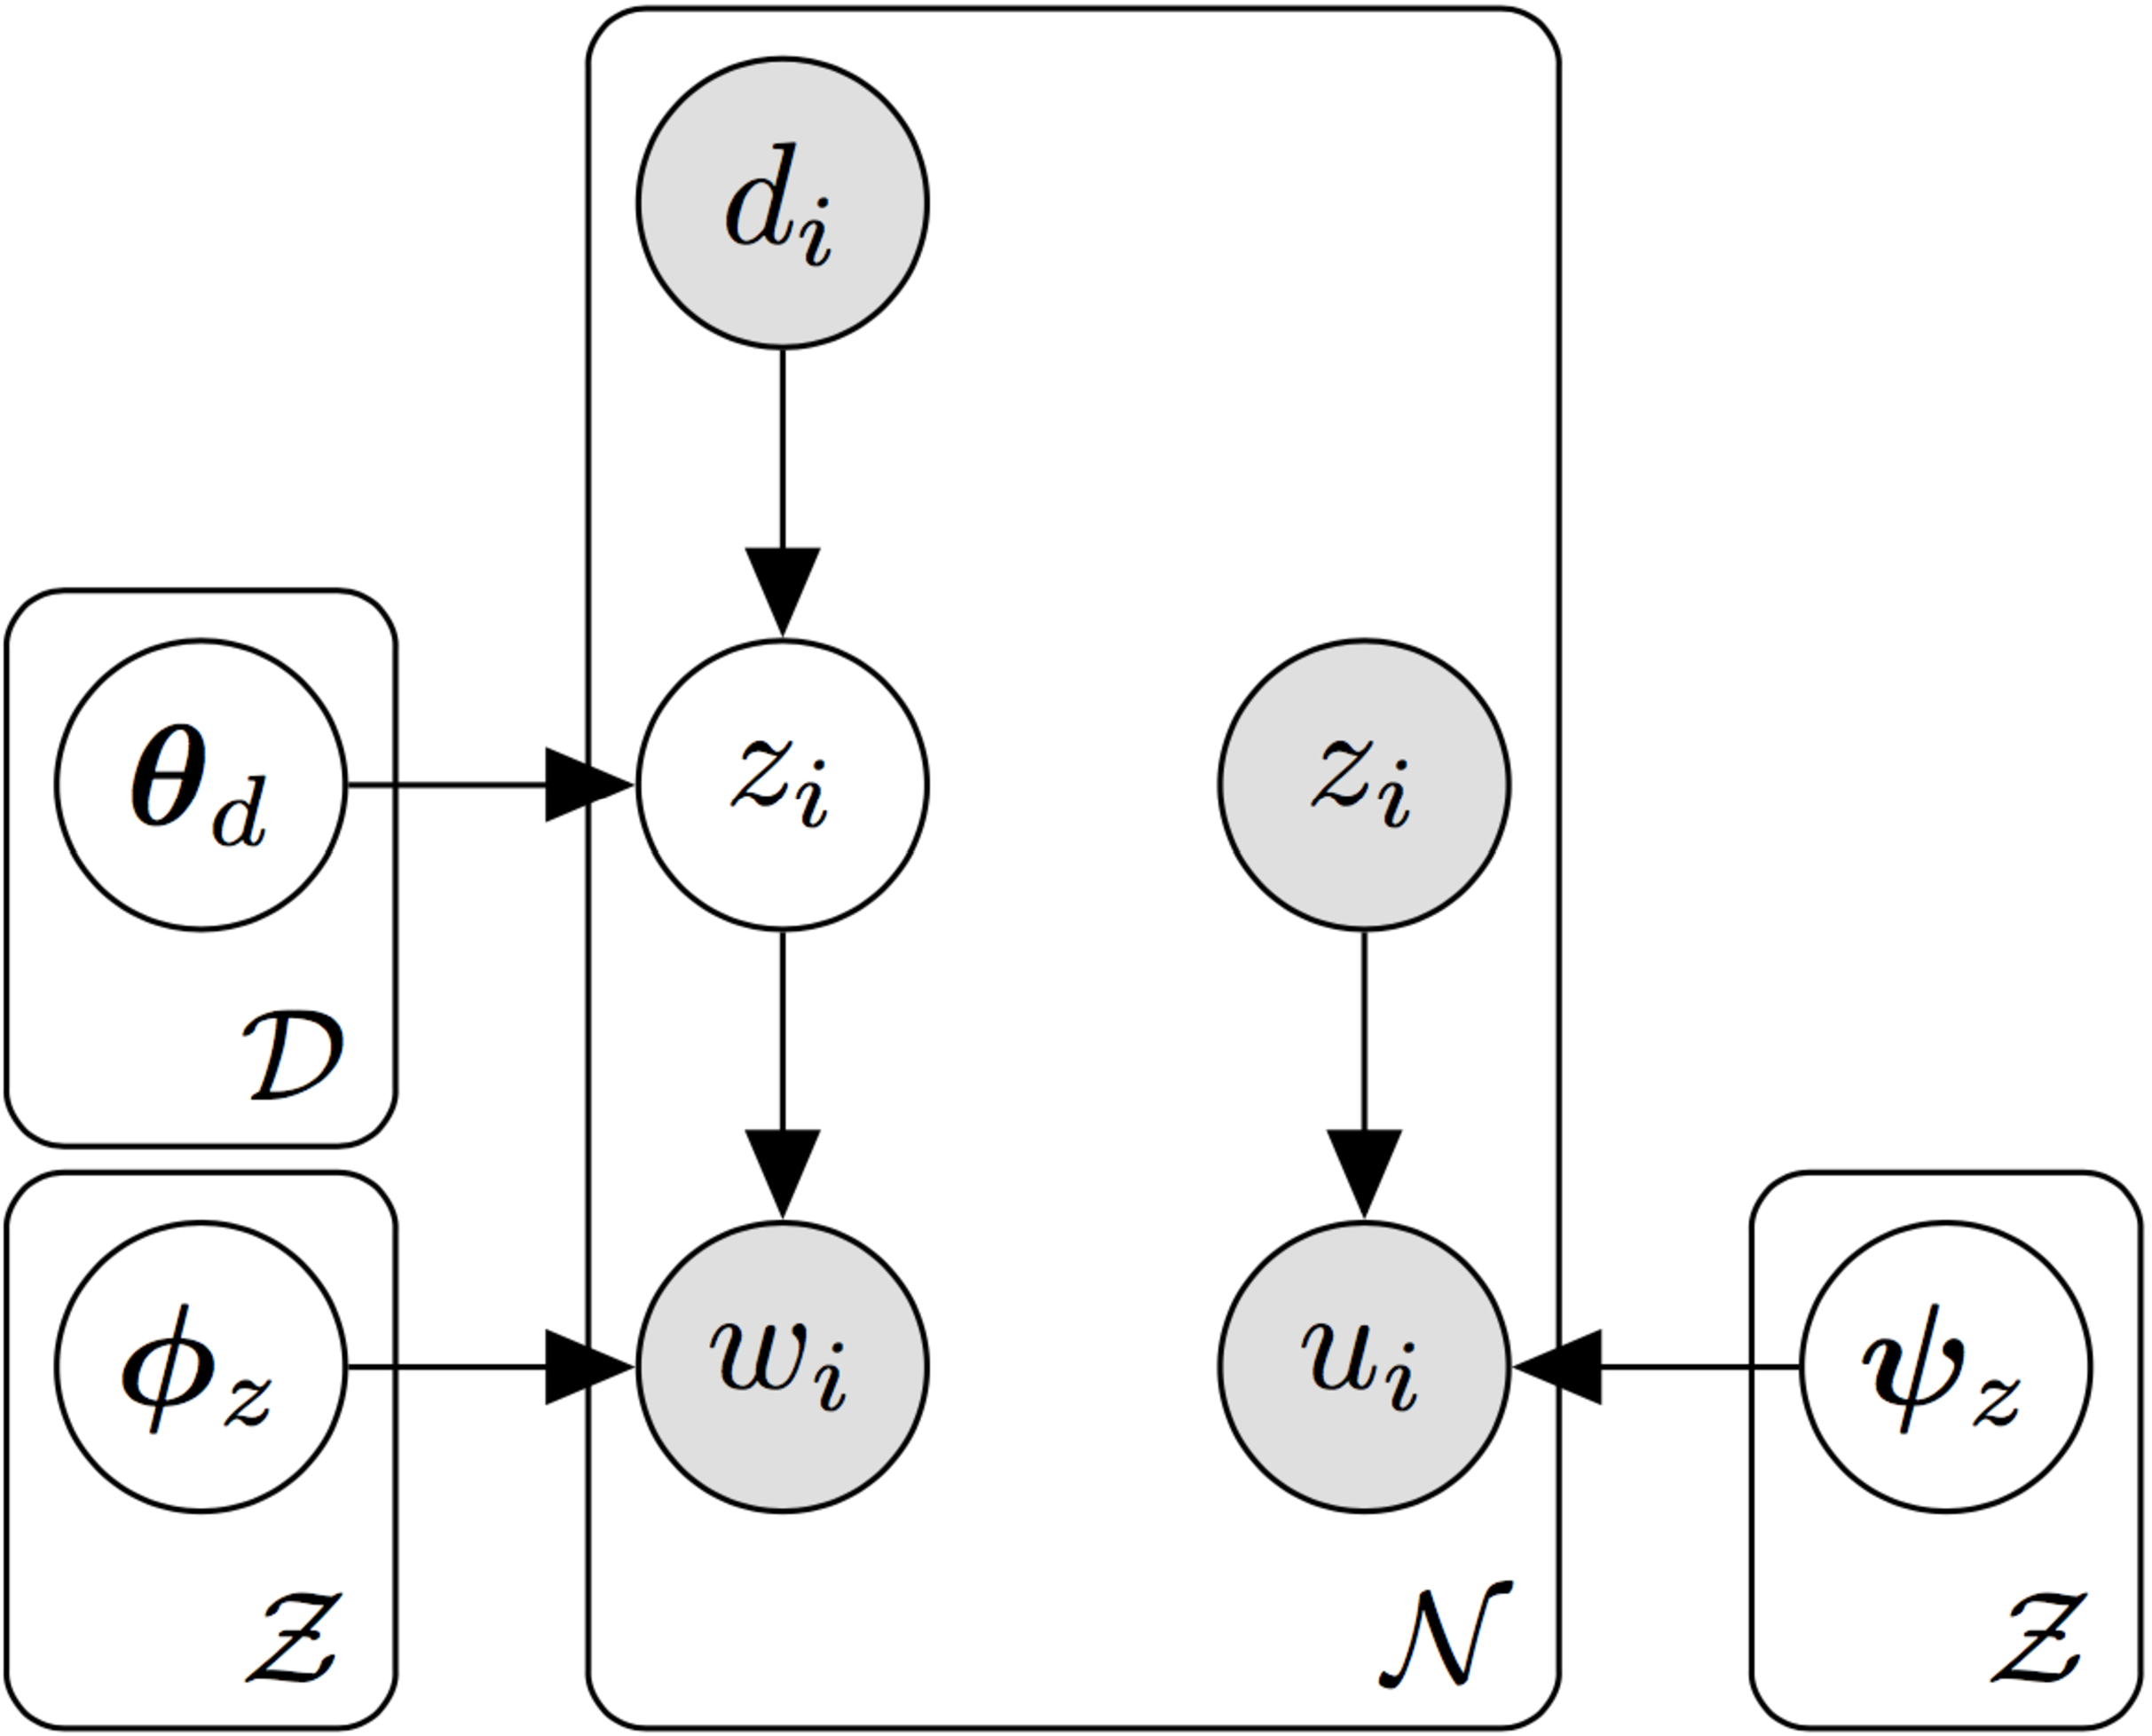
\includegraphics[width=0.8\linewidth]{figures/ptm-simplified}
  \caption{}
  \label{fig:ptm-simplified}
  \end{subfigure}
  \end{center}
  \caption{The proposed graphical model for personalized retrieval in Figure~\ref{fig:ptm-original} and the actual simplified model used for parameter estimation in Figure~\ref{fig:ptm-simplified} (both figures are from \cite{Harvey-2013}.)}
  \label{fig:ptm}
\end{figure}

As shown in Figure~\ref{fig:ptm-original}, instead of just two observed variable (document $d_i$ and query word $w_i$) as in normal topic models, this model adds one extra observed variable $u_i$ for user and directly estimate the probability of $p(k|w_i, d_i, u_i)$. They further assume the conditional independence among the word $w_i$, the user $u_i$ and document $d_i$ given the topic $k$, and the model can be simplified as,
\begin{align}
p(k \g w_i, d_i, u_i) = \frac{p(k,w_i, u_i  \g  d_i)}{p(w_i, u_i | d_i)} \propto p(w_i \g k) p(u_i \g k) p (k \g d_i)
\end{align}

By directly including the user in the topic model, this model assumes the user's topical interests for describing a document that the user clicked is equally important as the words to describe the document. This assumption is too strong as shown in \citet{Carman-2010}. As a result, \citet{Harvey-2013} further propose to not consider the user explicitly in the Markov chain topic sampling and simplify the model as shown in Figure~\ref{fig:ptm-simplified}. In this model, the topics are used to infer the topic-user distribution $p(u_i|k)$ once the Markov chain is converged. The intuition is to capture the idea that a user clicks on a document given a specific query due to his/her interests expressed over the topic space~\citep{Harvey-2013}.

Based on the estimates of this personalized topic model, the documents are ranked by the likelihood given the query and the user as follows,
\begin{align}
p(d  \g  q,u) &\propto p(d) \prod_{w \in q} p(w, u  \g  d)\\
&\propto p(d) \prod_{w \in q} \sum_k p(w \g k) p(u|k) p(k \g d) \notag
\end{align}
By subtly incorporating users' profiles as part of the ranking algorithms, \citet{Harvey-2013} significantly improved the personalized ranked document lists than the non personalized baselines.

\section{Conclusion}

Because topic models analyze documents on a semantic level, it offers
an interesting and unique framework for modeling the document-word
relations and word-word relations. As a result, topic models have been
successfully applied in smoothing language models, query expansion and search personalization.

There are also some works focusing on the diversification of the search results~\citep{Dang-2013,Santos-2015}. The goal of search result diversification is to identify the different aspects of the ambiguous query, retrieve documents for each aspect and make the search results more diverse~\citep{Dang-2013}. Similarly, the diversification techniques can also be further combined with personalization to diversify the personalized search results~\citep{Vallet-2012,Liang-2014}. This topic is beyond the scope of this chapter.

These successful applications on information retrieval are based on a general good
understanding of the outputs of topic models. In the next chapter, we
will introduce how to visualize and label the topics in general to
help the users better understand the topics.


%%%%%%%%%%%%%%%%%%%%%%%%%%%%%%%%%%%%%%%%%%%%%%%%%%%%%%%%%%%%%%%%%%%%%%%%%%%%%%%%%%%%%%%%%%%%%%%%%%%%%%%%%%%%%%%%%%%%%%%%%
%%%%%%%%%%%%%%%%%%%%%%%%%%%%%%%%%%%%%%%%%%%%%%%%%%%%%%%%%%%%%%%%%%%%%%%%%%%%%%%%%%%%%%%%%%%%%%%%%%%%%%%%%%%%%%%%%%%%%%%%%
%%%%%%%%%%%%%%%%%%%%%%%%%%%%%%%%%%%%%%%%%%%%%%%%%%%%%%%%%%%%%%%%%%%%%%%%%%%%%%%%%%%%%%%%%%%%%%%%%%%%%%%%%%%%%%%%%%%%%%%%%
%%%%%%%%%%%%%%%%%%%%%%%%%%%%%%%%%%%%%%%%%%%%%%%%%%%%%%%%%%%%%%%%%%%%%%%%%%%%%%%%%%%%%%%%%%%%%%%%%%%%%%%%%%%%%%%%%%%%%%%%%
%%%%%%%%%%%%%%%%%%%%%%%%%%%%%%%%%%%%%%%%%%%%%%%%%%%%%%%%%%%%%%%%%%%%%%%%%%%%%%%%%%%%%%%%%%%%%%%%%%%%%%%%%%%%%%%%%%%%%%%%%


\begin{comment}
\cite{PonteCroft} first propose the language model in information retrieval. They treat the generation of queries as a random process and use the probabilities from documents to model the query generations. However, they think the maximum likelihood estimator (Equation~\ref{eq:ir_mse}) is not accurate, given the limited size of a document. So they propose to use the averaged probability across the corpus to smooth the maximum likelihood estimator. The averaged probability $p_{\texttt{avg}}(t)$ is computed as,
\begin{align}
p_{\texttt{avg}}(t) = \frac{\sum_{d_{t \in d}} p_{\texttt{ml}}(t|d)}{\texttt{df}_t}
\end{align}
where $\texttt{df}_t$ is the document frequency of term $t$. They then combine the maximum likelihood estimator with this averaged probability across the corpus,
\begin{align}
p(t|d) &= p_{\texttt{ml}}(t|d)^{(1-R_{t,d})} \times p_{\texttt{avg}}(t)^{R_{t,d}}
\end{align}
where $R_{t,d}$ is the risk for a term $t$ in document $d$ using the geometric distribution, computed as,
\begin{align}
R_{t,d} &= (\frac{1}{1+\bar{f_t}}) \times (\frac{\bar{f}_t}{1+\bar{f}_t})^{\texttt{tf}_{t,d}} \\
\bar{f}_t &= \frac{\sum_{d_{t \in d}} \texttt{tf}_{t,d}}{\texttt{df}_t}
\end{align}
where $\texttt{tf}_{t,d}$ is the term frequency of term $t$ in document $d$; $\bar{f}_t$ is the mean term frequency of term $t$ in all documents where term $t$ occurs.

For the missing terms in the current document, \cite{PonteCroft} estimate their probabilities based on the ratio of the term frequency in all documents and the total number of tokens, normally referred as background probability. The final probability is estimated by,
\begin{align}
p(t|d) =
\begin{cases}
p_{\texttt{ml}}(t|d)^{(1-R_{t,d})} \times p_{\texttt{avg}}(t)^{R_{t,d}},~~~~~~~~&\text{if $tf_{t,d}$ > 0}\\
\frac{\sum_d \texttt{tf}_{t,d}}{\sum_{t} \sum_d \texttt{tf}_{t,d}}. &\text{otherwise}
\end{cases}
\end{align}

Following \cite{PonteCroft}, \cite{song-99} further explore the language models for information retrieval based on a range of data smoothing techniques. They first apply the Good-Turing estimate to smooth each document language model, which allocates some probability to the missing terms as,
\begin{align}
p_{\texttt{GT}}(t|d) = \frac{(tf+1)S(N_{tf+1})}{N_d S(N_{tf})}
\end{align}
where $tf$ is the term frequency of term $t$; $N_{tf}$ is the number of terms with frequency $tf$ in a document; $S(N_{tf})$ is a smoothed function.

The second approach that \cite{song-99} proposed is to expand a document model with the corpus model, which is very similar to the idea in \cite{PonteCroft}, except that they are using a weighted sum and a weight $w$ can be learned,
\begin{align}
p(t|d) = w \times p_{document}(t|d) + (1-w) \times p_{corpus}(t)
\end{align}

\cite{song-99} further propose to combine unigrams and bigrams to further smooth the probability,
\begin{align}
p(t_{i-1},t_i|d) = w \times p_1(t_i|d) + (1-w) \times p_2(t_{i-1},t_i | d)
\end{align}
which can be further extended to include trigrams as well.
\end{comment}



\begin{comment}

\chapter{Information Retrieval Structure}
\label{ch:ir_structure}

Topic models, such as Latent Semantic Analysis (LSA) by \citep{deerwester-90} and probabilistic Latent Semantic Indexing~\cite{hofmann-99a}, can capture the semantic relations between documents and queries~\citep{wei-07}.

Topic models have been applied into the information retrieval framework to improve ranking results. Probabilistic language modeling~\citep{croft-03} is a common formalism that incorporates information from topic models.

In this chapter, we briefly introduce the information retrieval framework and the semantic relations between queries and documents. We also present the latent semantic analysis and probabilistic latent semantic indexing models, and how they are combined into information retrieval framework through language modeling.

\section{Semantic Relations in Information Retrieval}

Information Retrieval (IR) systems aim to retrieve relevant documents by comparing query and document texts.

From computer's view, documents are usually treated as ``bags of words'', and documents are retrieved and ranked by measuring the word overlap. This is consistent with topic models.

Topic models use those bags of words to build abstractions (topics), however.

However, humans would use background knowledge to interpret and understand the queries and ``add'' missing words~\citep{wei-07}, akin to query expansion.

\jbgcomment{You never define what's a semantic relation here}

To more accurately retrieve related documents, the semantic relations between queries and documents are needed to improve the ranking results. Topic models, which describe each topic using weighted words and model each document as a distribution over all topics, is an effective way to capture such semantic relations~\citep{deerwester-90,hofmann-99a}.

\section{Topic Models in IR}

Latent Semantic Analysis (LSA) proposed by \citet{deerwester-90} makes use of dimensionality reduction to capture the semantic relations among words and documents.  (Briefly review, note distinction with probabilistic approaches.)

It has been successfully applied into the information retrieval systems through automatic indexing with LSA (Latent Semantic Indexing, LSI) \citep{deerwester-90,dumais-95}.

Probabilistic Latent Semantic Indexing (pLSI), introduced by \citet{hofmann-99a}, is an aspect model which associates an unobserved class (topic) variable with each observed word occurrence. pLSI provides a better fit to text data than LSI, thus quickly gained acceptance in IR systems.

\section{Applying Topic Models into IR}

The language modeling approach~\citep{croft-03,PonteCroft,song-99} is the main framework for using topic models in IR systems, since it has been shown to be effective probabilistic framework for studying information retrieval problems~\citep{PonteCroft,berger-99}.

The basic language modeling framework is to compute the model likelihood of documents for generating the queries. Topic models, which represent documents with topics, offer a new and interesting means to model documents~\citep{wei-07}. A probability mixture model and a term model with back-off smoothing are presented to integrate topic models in this section.

A probability mixture model combines multiple different probability distributions to integrate different factors in IR for query representation or document representation~\citep{miller-99,zhai-01,liu-04}.

A term model with back-off smoothing~\citep{katz-87} is another popular framework to use topic models in IR systems, where a term model is learned for each term in a document and the back-off smoothing~\citep{katz-87} is applied.

% Perhaps it would be nice to mention e-discovery?

Transition to next chapter: what if you care about recall and understanding

\end{comment}
